\documentclass[11pt]{article}
\usepackage{certmachine}
%% generated by tools/paper-numbers/matmul-records.js — do not edit (git eece01c1497a)
\newcommand{\RepoCommit}{eece01c1497a}
\newcommand{\CorpusRows}{11}
\newcommand{\CorpusVerified}{10}
\newcommand{\CorpusRejects}{1}
\newcommand{\CorpusEquations}{46{,}466}
\newcommand{\CorpusLiveMs}{32}
\newcommand{\CertGeneratedBy}{\path{tools/export-strassen-certificate.js} at git \texttt{1d2b452}}
\newcommand{\AERank}{48}
\newcommand{\AEScale}{8}
\newcommand{\AEEquations}{4{,}096}
\newcommand{\AELayout}{CA}
\newcommand{\AENaive}{64}
\newcommand{\AEPin}{\texttt{2cce2543e48c89aa}\ldots}
\newcommand{\AECommit}{\texttt{4226acb}}
\newcommand{\AEAlphabet}{9}
\newcommand{\AENonzero}{1{,}376}
\newcommand{\AEEntries}{2{,}304}
\newcommand{\ATRank}{47}
\newcommand{\ATEquations}{4{,}096}
\newcommand{\ATLayout}{CA}
\newcommand{\ATFiveRank}{96}
\newcommand{\ATFiveEquations}{15{,}625}
\newcommand{\ATFiveNaive}{125}
\newcommand{\ATPinF}{\texttt{70f09f349d8d2874}\ldots}
\newcommand{\ATPinR}{\texttt{4d59571a2537a947}\ldots}
\newcommand{\ATQFailAb}{0}
\newcommand{\ATQFailBc}{0}
\newcommand{\ATQFailK}{2}
\newcommand{\ATQFailSum}{2}
\newcommand{\ATQFailTarget}{0}
\newcommand{\ATQFailCount}{465}
\newcommand{\ATQFailPct}{11.4\%}
\newcommand{\ATQMaxAbs}{8}
\newcommand{\ATFiveQFailCount}{1{,}043}
\newcommand{\ATFiveQFailPct}{6.7\%}
\newcommand{\StrassenRank}{7}
\newcommand{\StrassenEquations}{64}
\newcommand{\StrassenSqRank}{49}
\newcommand{\StrassenSqEquations}{4{,}096}
\newcommand{\LadermanRank}{23}
\newcommand{\LadermanEquations}{729}
\newcommand{\ATQFourRank}{49}
\newcommand{\NaiveTwoRank}{8}
\newcommand{\ATQRows}{5}
\newcommand{\ATFRows}{2}
\newcommand{\RegistryRows}{\texttt{strassen-1969} & $2\times2\times2$ & 7 & 8 & $\Q$ & 64 & AC & VERIFIED & Strassen 1969, textbook transcription \\
\texttt{strassen-squared-4x4x4} & $4\times4\times4$ & 49 & 64 & $\Q$ & 4{,}096 & AC & VERIFIED & Strassen $\otimes$ Strassen, generated here \\
\texttt{naive-2x2x2} & $2\times2\times2$ & 8 & 8 & $\Q$ & 64 & AC & REJECT (correct, not fast) & the definition, generated here \\
\texttt{alphatensor-q-2x2x2} & $2\times2\times2$ & 7 & 8 & $\Q$ & 64 & CA & VERIFIED & AlphaTensor npz, key 2,2,2 \\
\texttt{alphatensor-q-3x3x3} & $3\times3\times3$ & 23 & 27 & $\Q$ & 729 & CA & VERIFIED & AlphaTensor npz, key 3,3,3 \\
\texttt{alphatensor-q-4x4x4} & $4\times4\times4$ & 49 & 64 & $\Q$ & 4{,}096 & CA & VERIFIED & AlphaTensor npz, key 4,4,4 \\
\texttt{alphatensor-q-3x4x5} & $3\times4\times5$ & 47 & 60 & $\Q$ & 3{,}600 & CA & VERIFIED & AlphaTensor npz, key 3,4,5 \\
\texttt{alphatensor-q-4x5x5} & $4\times5\times5$ & 76 & 100 & $\Q$ & 10{,}000 & CA & VERIFIED & AlphaTensor npz, key 4,5,5 \\
\texttt{alphatensor-f2-4x4x4} & $4\times4\times4$ & 47 & 64 & $\mathbb{F}_2$ & 4{,}096 & CA & VERIFIED; refuted over $\Q$ & AlphaTensor npz, key 4,4,4 \\
\texttt{alphatensor-f2-5x5x5} & $5\times5\times5$ & 96 & 125 & $\mathbb{F}_2$ & 15{,}625 & CA & VERIFIED; refuted over $\Q$ & AlphaTensor npz, key 5,5,5 \\
\texttt{alphaevolve-48-4x4x4} & $4\times4\times4$ & 48 & 64 & $\Z[i]$ & 4{,}096 & CA & VERIFIED & AlphaEvolve notebook @ 4226acb \\}
\newcommand{\VerifierEntries}{10}
\newcommand{\VerifierFailures}{0}
\newcommand{\StrassenBatteryChecks}{31}
\newcommand{\StrassenBatteryReds}{5}
\newcommand{\LBNodes}{496}
\newcommand{\LBConfirmed}{4}
\newcommand{\LBTight}{8}
\newcommand{\LBSurvives}{6}
\newcommand{\LBNotAttacked}{478}
\newcommand{\LBRefuted}{0}
\newcommand{\LBAttacked}{18}
\newcommand{\LBNotAttackedPct}{96.4\%}
\newcommand{\LBWitnesses}{0}
\newcommand{\CNodes}{10}
\newcommand{\CWitnessesOk}{10}
\newcommand{\CWitnesses}{10}
\newcommand{\CConfirmed}{3}
\newcommand{\CTight}{3}
\newcommand{\CSurvives}{1}
\newcommand{\CNotAttacked}{3}
\newcommand{\CRefuted}{0}
\newcommand{\LBSeconds}{2.9}
\newcommand{\LBPin}{\texttt{25595a883ce877ee}\ldots}
\newcommand{\CPin}{\texttt{27b0dc70d76e6405}\ldots}
\newcommand{\LBBatteryChecks}{12}
\newcommand{\LBBatteryReds}{3}
\newcommand{\WallRows}{$\langle2,2,2\rangle$ control (rank 7 optimal) & 10 & 10 / 10 & 3 & 3 & 1 & 3 & 0 \\
$\langle3,3,3\rangle$, the bound $\ge 20$ & 496 & --- & 4 & 8 & 6 & 478 & 0 \\}
\newcommand{\AddCounted}{55}
\newcommand{\AddDeclared}{55}
\newcommand{\AddRank}{23}
\newcommand{\AddBrent}{729}
\newcommand{\AddLayout}{AC}
\newcommand{\AddScalarOps}{78}
\newcommand{\AddNaive}{122}
\newcommand{\AddU}{13}
\newcommand{\AddV}{14}
\newcommand{\AddW}{28}
\newcommand{\AddNaiveU}{43}
\newcommand{\AddNaiveV}{30}
\newcommand{\AddNaiveW}{49}
\newcommand{\AddPin}{\texttt{91c36b1165a71d4b}\ldots}
\newcommand{\AddSourceDeclared}{58}
\newcommand{\AddSourceU}{14}
\newcommand{\AddSourceV}{15}
\newcommand{\AddSourceW}{29}
\newcommand{\AddSourcePath}{\texttt{3x3x3\_m23\_cr58\_cn122\_ZT\_reduced.json}}
\newcommand{\AddTransposition}{$14 + 23 - 9 = 28$}
\newcommand{\AddLocalLBU}{13}
\newcommand{\AddLocalLBV}{14}
\newcommand{\AddPartRows}{\texttt{U\_input} & form the 23 left factors from the 9 entries of A & 13 & 13 & 43 & exactly \\
\texttt{V\_input} & form the 23 right factors from the 9 entries of B & 14 & 14 & 30 & exactly \\
\texttt{W\_output} & combine the 23 products into the 9 entries of C & 28 & 28 & 49 & exactly \\
total & the whole linear cost & 55 & 55 & 122 & agree \\}
\newcommand{\SlpBatteryChecks}{16}
\newcommand{\SlpBatteryReds}{8}
\newcommand{\BLTargets}{9}
\newcommand{\BLBeat}{0}
\newcommand{\BLMatch}{3}
\newcommand{\BLAbove}{3}
\newcommand{\BLUnpublished}{3}
\newcommand{\BLTight}{1}
\newcommand{\BLEquations}{2{,}824}
\newcommand{\BLSeconds}{1{,}331}
\newcommand{\BLMinutes}{22}
\newcommand{\BLUntouched}{6}
\newcommand{\BLUntouchedList}{\texttt{P6}, \texttt{P7}, \texttt{P8}, \texttt{C10}, \texttt{T10}, \texttt{T11}}
\newcommand{\BLMatchList}{\texttt{C7}, \texttt{T6}, \texttt{T7}}
\newcommand{\BLAboveList}{\texttt{C8} (25 against 22), \texttt{T8} (23 against 22), \texttt{T9} (27 against 26)}
\newcommand{\BLPublishedRows}{12}
\newcommand{\BLRetrieved}{2026-08-30}
\newcommand{\CSevenRank}{13}
\newcommand{\CSevenNaive}{49}
\newcommand{\CSevenSeconds}{20}
\newcommand{\CEightRank}{25}
\newcommand{\CEightUpper}{22}
\newcommand{\CEightSeconds}{667}
\newcommand{\TNineRank}{27}
\newcommand{\TNineUpper}{26}
\newcommand{\TEightRank}{23}
\newcommand{\TEightUpper}{22}
\newcommand{\BLSeeds}{8 or 12}
\newcommand{\BLSteps}{300{,}000 or 800{,}000}
\newcommand{\BLRows}{\texttt{C7} & cyclic, $n=7$ & 49 & 13--13 & 13 & MATCH & Wagh--Morgera 1983 \\
\texttt{C8} & cyclic, $n=8$ & 64 & 19--22 & 25 & above & Morgera 1990; Cenk--\"Ozbudak 2011 \\
\texttt{P2} & full, $n=2$ & 4 & CK 3 & 3 & matches CK & Chen--Kauers 2025 table \\
\texttt{P3} & full, $n=3$ & 9 & CK 6 & 6 & matches CK & Chen--Kauers 2025 table \\
\texttt{P4} & full, $n=4$ & 16 & CK 9 & 9 & matches CK & Chen--Kauers 2025 table \\
\texttt{T6} & truncated, $n=6$ & 21 & 13--14 & 14 & MATCH & Cenk--\"Ozbudak 2011 \\
\texttt{T7} & truncated, $n=7$ & 28 & 16--18 & 18 & MATCH & Cenk--\"Ozbudak 2011 \\
\texttt{T8} & truncated, $n=8$ & 36 & 19--22 & 23 & above & Cenk--\"Ozbudak 2011 \\
\texttt{T9} & truncated, $n=9$ & 45 & 21--26 & 27 & above & Wang 2026, footnote \\}
\newcommand{\BLUntouchedRows}{\texttt{P6} & 16 & 15 & 17 & Montgomery 2005 \\
\texttt{P7} & 19 & 18 & 22 & Montgomery 2005 \\
\texttt{P8} & 21 & 20 & 26 & Winograd 1977; Fan--Hasan 2007 \\
\texttt{C10} & 22 & 19 & 29 & Morgera 1990 \\
\texttt{T10} & 24 & 20 & 31 & Cenk--\"Ozbudak 2011 \\
\texttt{T11} & 27 & 22 & 36 & Cenk--\"Ozbudak 2011 \\}
\newcommand{\BLBatteryChecks}{16}
\newcommand{\BLBatteryReds}{8}
\newcommand{\BLBatteryLadder}{4}
\newcommand{\EARows}{20}
\newcommand{\EAProblems}{8}
\newcommand{\EAWitnessed}{16}
\newcommand{\EARepaired}{4}
\newcommand{\EAUnwitnessed}{0}
\newcommand{\EAImprovements}{8}
\newcommand{\EAFiles}{36}
\newcommand{\EACommit}{\texttt{c388c6f7}}
\newcommand{\EAFetched}{2026-09-08}
\newcommand{\EAGenerated}{2026-09-16}
\newcommand{\EARepo}{\path{github.com/togethercomputer/EinsteinArena-new-SOTA}}
\newcommand{\EAUndecided}{2}
\newcommand{\EAPrinted}{19}
\newcommand{\EAPrintedAgree}{18}
\newcommand{\EALargestExact}{$2.6\times10^{-4}$}
\newcommand{\EASmallest}{$9.06\times10^{-9}$}
\newcommand{\EALargest}{$6.00\times10^{-2}$}
\newcommand{\CirPairs}{44}
\newcommand{\CirAllPairs}{210}
\newcommand{\CirWorst}{$3.09\times10^{-12}$}
\newcommand{\CirWorstPair}{3--17}
\newcommand{\CirBox}{$4.20\times10^{-14}$}
\newcommand{\CirLambda}{0.999999999963354125\ldots}
\newcommand{\CirLambdaDeficit}{$3.66\times10^{-11}$}
\newcommand{\CirSumPublished}{2.3658323759185154}
\newcommand{\CirSumRepaired}{2.3658323758318174}
\newcommand{\CirDeficit}{$8.67\times10^{-11}$}
\newcommand{\CirPrinted}{2.3658323759}
\newcommand{\CirRepairRounded}{2.3658323758}
\newcommand{\CirAEWorst}{$5.04\times10^{-9}$}
\newcommand{\CirAEBox}{$3.20\times10^{-8}$}
\newcommand{\CirAEPrinted}{2.3658321334}
\newcommand{\CirAEExact}{2.3658321334167631}
\newcommand{\CirImprovement}{$2.42\times10^{-7}$}
\newcommand{\OvMissMin}{$1.0\times10^{-15}$}
\newcommand{\OvMissMax}{$1.5\times10^{-14}$}
\newcommand{\OvDeltaMax}{$8.3\times10^{-18}$}
\newcommand{\OvTPrinted}{0.380876}
\newcommand{\OvTExact}{0.3808753232}
\newcommand{\OvOPrinted}{0.380871}
\newcommand{\OvOExact}{0.3808703105}
\newcommand{\OvHSteps}{51}
\newcommand{\OvOSteps}{600}
\newcommand{\OvImprovement}{$5.01\times10^{-6}$}
\newcommand{\AcN}{30{,}000}
\newcommand{\AcCandidates}{10}
\newcommand{\AcArgmax}{28{,}879}
\newcommand{\AcScreen}{$2.7\times10^{-11}$}
\newcommand{\AcExact}{1.5028628587049711}
\newcommand{\AcPrinted}{1.50286286}
\newcommand{\AcTExact}{1.502862898255\ldots}
\newcommand{\AcTPrinted}{1.50286290}
\newcommand{\AcVN}{1{,}319}
\newcommand{\AcVExact}{1.5031635546\ldots}
\newcommand{\AcImprovement}{$3.96\times10^{-8}$}
\newcommand{\FlDegree}{69}
\newcommand{\FlLo}{1.280932052875041675}
\newcommand{\FlHi}{1.280932052875041753}
\newcommand{\FlWidth}{$7.8\times10^{-17}$}
\newcommand{\FlGrid}{1.2809320527987995}
\newcommand{\FlShortfall}{$7.62\times10^{-11}$}
\newcommand{\FlPrinted}{1.280932}
\newcommand{\FlCrit}{43}
\newcommand{\FlMs}{403}
\newcommand{\FlAELo}{1.3409252804007615}
\newcommand{\FlAEHi}{1.3409252804007616}
\newcommand{\FlAEShortfall}{$9.45\times10^{-10}$}
\newcommand{\FlAEPrinted}{1.340925}
\newcommand{\FlAECrit}{39}
\newcommand{\FlImprovement}{$6.00\times10^{-2}$}
\newcommand{\HxPairs}{66}
\newcommand{\HxVertices}{72}
\newcommand{\HxGap}{$3.6\times10^{-8}$}
\newcommand{\HxAEGap}{$6.9\times10^{-6}$}
\newcommand{\HxCross}{$4.1\times10^{-7}$}
\newcommand{\HxWidth}{$6.2\times10^{-15}$}
\newcommand{\HxSide}{3.9416523}
\newcommand{\HxAESide}{3.9419123}
\newcommand{\HxImprovement}{$2.6\times10^{-4}$}
\newcommand{\HxPlatformTol}{a pair counts as intersecting unless separated by more than 1e-9; a vertex counts as inside unless outside by more than 1e-9}
\newcommand{\EdImprovement}{$2.38\times10^{-4}$}
\newcommand{\EdPrinted}{-0.712256}
\newcommand{\EdExact}{-0.712256332697931}
\newcommand{\HbImprovement}{$9.06\times10^{-9}$}
\newcommand{\MdImprovement}{$3.62\times10^{-5}$}
\newcommand{\EATableRows}{circles in a rectangle & AlphaEvolve V2, 2025-11 & $2.3658321334$ & $2.3658321334167631$ & WITNESSED & the exact value's rounding \\
circles in a rectangle & Together AI agents, 2026-04 & $2.3658323759$ & $2.3658323758318174$ & REPAIRED & NOT the witness's rounding \\
Heilbronn, convex region & AlphaEvolve V2, 2025-11 & $0.0278355715$ & $0.0278355714584821$ & WITNESSED & the exact value's rounding \\
Heilbronn, convex region & Together AI agents, 2026-04 & $0.0278355805$ & $0.0278355805175536$ & WITNESSED & the exact value's rounding \\
min-distance ratio, 2-D & AlphaEvolve, 2025-06 & $12.889266$ & $12.8892661120346322$ & WITNESSED & the exact value's rounding \\
min-distance ratio, 2-D & Together AI agents, 2026-03 & $12.889230$ & $12.8892299077175173$ & WITNESSED & the exact value's rounding \\
Erd\H{o}s minimum overlap & Haugland, 2016 & $0.380927$ & $0.3809268534330869$ & WITNESSED & the exact value's ceiling \\
Erd\H{o}s minimum overlap & AlphaEvolve, 2025-06 & $0.380924$ & $0.3809230351084501$ & REPAIRED & the exact value's ceiling \\
Erd\H{o}s minimum overlap & TTT-Discover, 2026-01 & $0.380876$ & $0.3808753232177187$ & REPAIRED & the exact value's ceiling \\
Erd\H{o}s minimum overlap & Together AI agents, 2026-03 & $0.380871$ & $0.3808703105862199$ & REPAIRED & the exact value's ceiling \\
edges vs triangles & AlphaEvolve V2, 2025-11 & $-0.712494$ & $-0.7124938782214395$ & WITNESSED & the exact value's rounding \\
edges vs triangles & Together AI agents, 2026-03 & $-0.712256$ & $-0.7122563326979318$ & WITNESSED & the exact value's rounding \\
first autocorrelation & AlphaEvolve, 2025-06 & $1.50529397$ & $1.5052939684401608$ & WITNESSED & the exact value's ceiling \\
first autocorrelation & AlphaEvolve V2, 2025-11 & --- & $1.5031635546815609$ & WITNESSED & none printed \\
first autocorrelation & TTT-Discover, 2026-01 & $1.50286290$ & $1.5028628982558265$ & WITNESSED & the exact value's ceiling \\
first autocorrelation & Together AI agents, 2026-03 & $1.50286286$ & $1.5028628587049711$ & WITNESSED & the exact value's ceiling \\
flat polynomial & AlphaEvolve V2, 2025-11 & $1.340925$ & $1.3409252804007615$ & WITNESSED & the supremum's rounding \\
flat polynomial & Together AI agents, 2026-03 & $1.280932$ & $1.2809320528750416$ & WITNESSED & the supremum's rounding \\
hexagons in a hexagon & AlphaEvolve V2, 2025-11 & $3.9419123$ & $3.9419123000000000$ & WITNESSED & exact decimal; packing certified \\
hexagons in a hexagon & Together AI agents, 2026-04 & $3.9416523$ & $3.9416523000000000$ & WITNESSED & exact decimal; packing certified \\}
\newcommand{\EAImprovementRows}{circles in a rectangle & maximise & AlphaEvolve V2 & $2.42\times10^{-7}$ & ours taken as its REPAIRED exact witness \\
Heilbronn, convex region & maximise & AlphaEvolve V2 & $9.06\times10^{-9}$ &  \\
min-distance ratio, 2-D & minimise & AlphaEvolve & $3.62\times10^{-5}$ &  \\
Erd\H{o}s minimum overlap & minimise & TTT-Discover & $5.01\times10^{-6}$ &  \\
edges vs triangles & maximise & AlphaEvolve V2 & $2.38\times10^{-4}$ &  \\
first autocorrelation & minimise & TTT-Discover & $3.96\times10^{-8}$ &  \\
flat polynomial & minimise & AlphaEvolve V2 & $6.00\times10^{-2}$ & a lower bound on the difference: the two certified enclosures are disjoint \\
hexagons in a hexagon & minimise & AlphaEvolve V2 & $2.60\times10^{-4}$ & both outer sides are exact decimals; both packings certified as witnesses \\}
\newcommand{\EAUndecidedRows}{prime-number-theorem & S(f) = 0.994179 (AlphaEvolve: 0.921292) & NOT DECIDABLE AS STATED & the platform's score is estimated from 10,000,000 random samples; a Monte Carlo score is not a mathematical claim about the construction and this ledger does not certify it. \\
tammes / second \& third autocorrelation / uncertainty (README rows) & four further table rows & NEEDS DATA & the repository README lists them; no solution files are published in the repository at the pinned commit. \\}
\newcommand{\EABatteryChecks}{40}
\newcommand{\EABatteryReds}{14}
\newcommand{\EAGrammarW}{the bytes are an exact witness of the value stated}
\newcommand{\EAGrammarR}{a witness only up to the platform's tolerance; an exact witness built from the same bytes, its deficit printed}
\newcommand{\EAGrammarU}{the bytes fail exactly and no repair was built --- a finding about the bytes, never a refutation of the bound}

\setlength{\emergencystretch}{1.5em}

\newcommand{\F}{\mathbb{F}}
\newcommand{\mm}[3]{\langle #1,#2,#3\rangle}

\title{AI-era matrix-multiplication records, decided from their bytes:\\
AlphaEvolve, AlphaTensor, the EinsteinArena table,\\
the $3\times3$ addition count and the rank walls}
\author{\cmauthor}
\date{October 2026 --- draft v0.1 for review; every number interpolated from the record; machine-derived, not peer-reviewed; author list to be agreed}

\begin{document}
\maketitle

\begin{abstract}
A fast matrix-multiplication algorithm is a finite exact object: a rank-$R$ decomposition of the
matrix-multiplication tensor, three coefficient matrices whose defining identity, the Brent equations,
either holds over a stated ring or does not. We re-decide, from bytes pinned by digest and sharing no code
with any producer, the records that AI systems have set or claimed around this object and its neighbours.
AlphaEvolve's rank-\AERank\ $\mm444$ decomposition is certified over $\Z[i]$: all \AEEquations\ equations
hold exactly once the half-Gaussian denominators are cleared. AlphaTensor's rank-\ATRank\ $\mm444$ is
certified over $\F_2$, and the same factors fail over $\Q$ at \ATQFailCount\ of the \ATEquations\ equations:
the ring is part of the claim. Both walls of the rank of $\mm333$ are re-decided: a rank-\LadermanRank\
witness as a certificate, and, of the \LBNodes\ nodes of Wang's 2026 certificate for the lower bound $20$
over $\F_2$, \LBAttacked\ are attacked by an instrument that computes the true rank of each sub-tensor
rather than re-running the author's inference rules, \LBConfirmed\ proved two-sided, \LBRefuted\ refuted,
\LBNotAttacked\ beyond the instrument. The July 2026 claim of \AddCounted\ additions around a rank-\AddRank\
scheme is re-derived gate by gate ($\AddU+\AddV+\AddW$) together with its \AddBrent\ Brent equations. A free
flip-graph walk over $\F_2$ reproduces \BLMatch\ published polynomial-multiplication bounds, one of them
tight, and beats none. And the EinsteinArena ``new state of the art'' table, \EARows\ constructions on
\EAProblems\ problems, is read as the exact rationals its decimals denote: \EAWitnessed\ exact witnesses,
\EARepaired\ repaired within the platform's tolerance, no failure, all \EAImprovements\ improvements positive,
one printed digit that belongs to the tolerance, and a grid maximum replaced by a certified supremum. No bound
is improved. The contribution is the decision grammar --- verdict, witness, refusal as a result --- and a
public record that re-runs in seconds.
\end{abstract}

\section{Introduction}

Strassen multiplied two $2\times2$ matrices in seven multiplications \cite{St69}; Winograd proved seven
optimal \cite{Wi71}; Laderman multiplied $3\times3$ matrices in $23$ \cite{La76}, and no one has done better
since. Brent wrote the problem as a system of polynomial equations in the coefficients of a bilinear
algorithm \cite{Br70}, which is the form in which every claim below is decided. The lower bound for
$3\times3$ stood at $19$ from Bl\"aser's 2003 argument \cite{Bl03} until March 2026, when Wang's automated
method raised it to $20$ over $\F_2$ \cite{Wa26}. Two AI systems entered the upper-bound side: AlphaTensor
\cite{Fa22} produced, among other factorisations, a rank-$47$ algorithm for $4\times4$ matrices in modular
arithmetic, and AlphaEvolve \cite{No25} a rank-$48$ algorithm over the complex numbers, presented as an
improvement on the recursive Strassen rank $49$. Flip-graph search \cite{KM22} is now the standard
non-learned competitor, and has been pointed at polynomial multiplication \cite{CK25}. The additive cost of
Laderman-rank schemes became an active record in 2025--26, ending (for now) at $55$ additions \cite{KI26}.
And a platform, EinsteinArena, published a table of constructions on classical extremal problems claimed to
beat AlphaEvolve's, each checked by the platform's own floating-point verifier with tolerances \cite{EA26}.

Every one of these results was verified by its producer. The platform scores in floating point with stated
tolerances; the DeepMind notebook verifies its own decomposition in a cell; the lower-bound certificate was
checked by the code that produced it. None of that is a defect, but it leaves a specific gap: no independent
party had decided these objects in exact arithmetic, from the bytes as published, with a stated verdict
grammar and a record anyone can re-run. This paper fills that gap for the objects named in the title and
reports what was found, including the two findings that are not confirmations: a printed digit that belongs
to a tolerance rather than to a witness, and a benchmark score that is a grid maximum standing in for a
supremum. Nothing here improves a bound; a REPAIRED construction is not a refutation; a lower-bound node not
attacked is not a doubt. The novelty claimed is the grammar in which each object is decided and the record
underneath it, not the arithmetic, which is elementary throughout.

The kissing-number rows of the same platform's table are decided in a separate paper \cite{Kiss} and are
not repeated here.

\section{The object, the ring, and the grammar}\label{sec:object}

Let $A$ be $n\times m$ and $B$ be $m\times p$. Index the entries of $A$ by $ab = a\cdot m+b$, those of $B$
by $bc = b\cdot p+c$, and those of $C=AB$ by an index $k$ under one of two layouts, AC with
$k = a\cdot p + c$ or CA with $k = c\cdot n + a$. A bilinear algorithm of rank $R$ over a ring $\mathcal R$
is a triple of matrices $U\in\mathcal R^{nm\times R}$, $V\in\mathcal R^{mp\times R}$,
$W\in\mathcal R^{np\times R}$, run as
\[
L_t=\sum_{ab}U_{ab,t}A_{ab},\qquad R_t=\sum_{bc}V_{bc,t}B_{bc},\qquad C_k=\sum_{t=1}^{R}W_{k,t}\,L_tR_t .
\]
It is correct for every pair of matrices over $\mathcal R$ exactly when the one finite identity
\begin{equation}\label{eq:brent}
\sum_{t=1}^{R}U_{ab,t}\,V_{b'c,t}\,W_{k,t}\;=\;[\,b=b'\,]\cdot[\,k=\operatorname{idx}(a,c)\,]
\qquad\text{for all } ab,\ b'c,\ k
\end{equation}
holds: $nm\cdot mp\cdot np$ equations, each an exact sum of $R$ products (the Brent equations
\cite{Br70}). The layout is a publishing convention, not mathematics; the instrument tries both and records
the one under which \eqref{eq:brent} holds, and fails a claim only when it holds under neither.

\paragraph{Exactness.} Every published coefficient here is a small integer, so each sum in
\eqref{eq:brent} is bounded by $R\cdot\max|U|\cdot\max|V|\cdot\max|W|$; the instrument checks that this bound
lies below $2^{53}$ before summing in doubles, which are then exact, and its battery cross-checks a full audit
against an arbitrary-precision evaluation. Anything past the bound is refused, never approximated. Over
$\F_2$ a sum is a parity. Over $\Z[i]$ a coefficient is a pair of integers and a claim may carry an integer
scale $s$: the identity decided is $\sum_t U_{ab,t}V_{b'c,t}W_{k,t} = s\cdot[b=b'][k=\operatorname{idx}]$
with imaginary part exactly zero. This is the natural home of a decomposition published over
$\tfrac12\Z[i]$: doubling the factors clears the denominators and the claim becomes $\sum(2u)(2v)(2w)=8T$.

\paragraph{The word \emph{certified}.} We say that a claim is \emph{certified} when its defining finite
identity has been decided in exact arithmetic over the stated ring, from bytes pinned by their SHA-256
digest, by an instrument of this repository whose red controls (planted forgeries that must be refuted) fire
in the same run. Everywhere else we write \emph{decided} for the act and \emph{verified} or \emph{refuted}
for the outcome; ``proved'' is reserved for statements with a proof in the usual sense. The grammar of a
verdict is fixed per instrument and stated with it below: for a decomposition, VERIFIED, REFUTED (with the
first failing equation named), REJECT (the identity holds but the rank is not below the naive $nmp$), and
REFUSED (not decidable as given: a failed pin, a bound past exactness). A refusal is a result and is
reported as one.

\paragraph{Statement of results.} The following are decided on the machine that built this document, at
repository commit \texttt{\RepoCommit}, from the records named in the reproduction section.

\begin{proposition}[AlphaEvolve]\label{prop:ae}
The rank-\AERank\ $\mm444$ decomposition in the DeepMind notebook pinned at commit \AECommit\ (digest
\AEPin) satisfies \eqref{eq:brent} over $\Z[i]$ with scale $\AEScale$ under layout \AELayout: all
\AEEquations\ equations hold exactly, every imaginary part vanishing. It is certified; its rank is below
the generated Strassen$\,\otimes\,$Strassen rank \StrassenSqRank, itself re-decided from scratch.
\end{proposition}

\begin{proposition}[AlphaTensor, both rings]\label{prop:at}
The rank-\ATRank\ $\mm444$ factors of the pinned \texttt{alphatensor\_f2.npz} (digest \ATPinF) satisfy
\eqref{eq:brent} over $\F_2$ (all \ATEquations\ equations, layout \ATLayout) and are certified there. The
same factors, read as integers, fail \eqref{eq:brent} over $\Q$ at \ATQFailCount\ of the \ATEquations\
equations (\ATQFailPct), the first at $(ab,b'c,k)=(\ATQFailAb,\ATQFailBc,\ATQFailK)$ with sum \ATQFailSum\
where \ATQFailTarget\ is required. The rank-\ATFiveRank\ $\mm555$ factors of the same file behave the same
way: certified over $\F_2$, failing over $\Q$ at \ATFiveQFailCount\ of \ATFiveEquations\ equations.
\end{proposition}

\begin{proposition}[the $3\times3$ walls]\label{prop:walls}
A rank-\LadermanRank\ $\mm333$ decomposition (AlphaTensor's, from the pinned \texttt{alphatensor\_r.npz},
digest \ATPinR) is certified over $\Q$: all \LadermanEquations\ equations hold. Of the \LBNodes\ nodes of
Wang's certificate for $R_{\F_2}(\mm333)\ge20$ (digest \LBPin, which equals the git-lfs object id the author
published), \LBAttacked\ were attacked by computing the true minimum rank of the node's constrained
sub-tensor over $\F_2$: \LBConfirmed\ are proved two-sided, \LBTight\ carry an upper bound equal to the
claimed lower bound, \LBSurvives\ survive a search for a cheaper decomposition, and \LBRefuted\ are
refuted. \LBNotAttacked\ nodes (\LBNotAttackedPct) are beyond the instrument and rest on the author's
reasoning.
\end{proposition}

\begin{proposition}[the addition count]\label{prop:add}
The certificate of Karunaratne and Idamekorala \cite{KI26} (digest \AddPin) is verified: its three
straight-line programs compute exactly the factor matrices they claim, with $\AddU$, $\AddV$ and $\AddW$
gates, $\AddCounted$ in all, as declared; every coefficient is in $\{-1,0,1\}$; and the factor matrices
satisfy all \AddBrent\ Brent equations over $\Q$ (layout \AddLayout) at rank \AddRank.
\end{proposition}

\begin{proposition}[polynomial multiplication over $\F_2$]\label{prop:bl}
\BLTargets\ bilinear schemes found by a free flip-graph walk are certified over $\F_2$ against targets
rebuilt by literal polynomial arithmetic. Against the published table, \BLMatch\ match the best known upper
bound (\BLMatchList; \texttt{C7} is tight), \BLAbove\ land above it, \BLBeat\ beat it, and \BLUnpublished\
match the Chen--Kauers full-product table.
\end{proposition}

\begin{proposition}[the EinsteinArena table]\label{prop:ea}
Of the \EARows\ constructions the repository publishes at commit \EACommit, every one read as the exact
rationals its decimal literals denote, \EAWitnessed\ are exact witnesses of the value stated, \EARepaired\
are witnesses only within the platform's tolerance and are repaired from their own bytes, and \EAUnwitnessed\
fail. All \EAImprovements\ improvements over the previous best are positive exact differences, from
\EASmallest\ to \EALargest. Of \EAPrinted\ printed values, \EAPrintedAgree\ are the exact value's rounding
or ceiling; the one exception is the tolerance's digit.
\end{proposition}

\section{The registry: AlphaTensor and AlphaEvolve}\label{sec:registry}

Table~\ref{tab:registry} is the corpus of \texttt{families/strassen-audit}, re-certified in-process while
this document's macros were written (\CorpusLiveMs\ ms for all \CorpusRows\ rows, every source pin
re-hashed): \CorpusVerified\ verified rows holding \CorpusEquations\ equations between them, and
\CorpusRejects\ honest reject. Strassen's 1969 scheme, transcribed from the textbook, is the calibration;
Strassen$\,\otimes\,$Strassen is generated by exact Kronecker composition and re-decided as a fresh claim;
the naive rank-\NaiveTwoRank\ algorithm, the definition itself, certifies as correct and is REJECTED because a
hit asserts a rank strictly below $nmp$. Correct is not fast. The \ATQRows\ AlphaTensor rows over $\Q$ and
\ATFRows\ over $\F_2$ are converted mechanically from the two pinned \texttt{npz} files of the DeepMind
repository; the C-index layout differs between Strassen's transcription (AC) and the npz factors (CA), and
the audit detects it rather than assuming it.

\begin{table}[h]\centering\small
\resizebox{\linewidth}{!}{\begin{tabular}{llrrlrlll}\toprule
row & shape & rank & naive & ring & equations & layout & verdict & source \\\midrule
\RegistryRows
\bottomrule\end{tabular}}
\caption{Every row of the fast-matmul corpus, re-decided from pinned bytes. ``Naive'' is $nmp$, the
schoolbook count; ``equations'' is $nm\cdot mp\cdot np$, every one decided exactly.}\label{tab:registry}
\end{table}

\begin{figure}[h]\centering
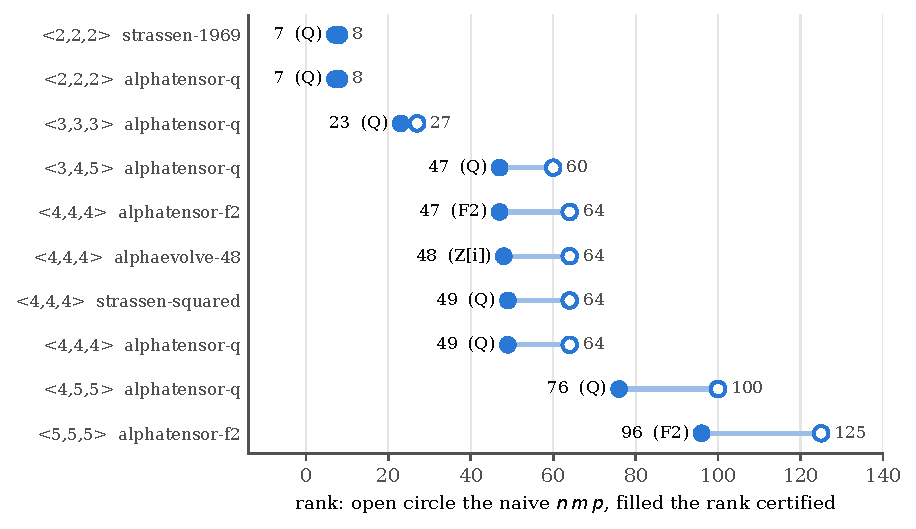
\includegraphics[width=\linewidth]{fig/matmul-records-ranks.pdf}
\caption{The ten verified rows, each drawn from the naive rank of its shape to the rank certified, with the
ring beside it. The ring is not decoration: the two $\F_2$ rows are refuted over $\Q$.}\label{fig:ranks}
\end{figure}

\paragraph{AlphaEvolve's 48, from mutable bytes.} The only first-party byte source for AlphaEvolve's
decomposition is a Jupyter notebook in a DeepMind repository whose main branch has been rewritten since
the result was announced; the arXiv paper \cite{No25} carries no ancillary files and is the citation, not
the source. The audit therefore pins by commit: the notebook is held at digest \AEPin, re-hashed at every
certify, and the row refuses if a byte moves. Every published entry lies in $\tfrac12\Z[i]$ --- the doubled
factors use \AEAlphabet\ distinct coefficients from $\{0,\pm1,\pm i,\pm1\pm i\}$, \AENonzero\ of the
\AEEntries\ entries non-zero --- and $\pm\tfrac12$ is exact in the notebook's \texttt{float32}, so the
byte-level parse loses nothing. The certified claim is the scale-\AEScale\ identity of
Proposition~\ref{prop:ae}. Its converter audits the claim before writing the corpus row, so a mis-parse
cannot land in the record; the row is then decided again, from the record, by the family.

\paragraph{AlphaTensor's 47, decided both ways.} The Nature paper says that its rank-\ATRank\ $4\times4$
algorithm works in modular arithmetic \cite{Fa22}. The audit turns that statement into a decided pair: the
same pinned factors are verified over $\F_2$ and refuted over $\Q$, with the failing equations located
(Proposition~\ref{prop:at}). Every one of the \ATEquations\ integer sums agrees with its target modulo $2$,
as it must, and \ATQFailCount\ of them differ as integers, by as much as \ATQMaxAbs. The speedup over
Strassen$\,\otimes\,$Strassen's \StrassenSqRank\ therefore does not survive lifting to characteristic zero
--- a statement about the published artifact, produced mechanically, of a kind a benchmark run cannot make,
since running the algorithm on integer matrices would return answers that are wrong and correct modulo $2$.
The AlphaTensor $\mm444$ factors over $\Q$ in the same release have rank \ATQFourRank, the Strassen-squared
rank, and are verified as such. We do not call the $\F_2$ refutation a correction of anything: the paper
states the ring; the record now decides it.

\paragraph{Independence.} The whole corpus detaches to \path{certs/strassen-certificate.json}, and
\path{tools/verify_strassen.py}, written against the standard library only and sharing no line with the
instrument, re-decides every entry from the file alone: \VerifierEntries\ entries, \VerifierFailures\
failures, and a red control that forges one coefficient by $+1$ and must be refuted before the script exits
green. The instrument's own battery runs \StrassenBatteryChecks\ checks with \StrassenBatteryReds\ red
controls.

\section{The rank walls of $\mm333$}\label{sec:walls}

The rank of $3\times3$ matrix multiplication is the oldest open interval in the subject: the upper wall is
Laderman's \LadermanRank\ \cite{La76}, the lower wall was Bl\"aser's $19$ for twenty-three years
\cite{Bl03}. Wang's preprint \cite{Wa26} raises the lower wall to $20$ over $\F_2$ by an automated
case split whose proof is a machine-checkable certificate: \LBNodes\ nodes, each a constrained sub-tensor
with a claimed lower bound derived by one of four inference rules. So far as we could establish, that
certificate had not been independently checked. (Bl\"aser's $19$ is a statement over any field; the $20$ is
an $\F_2$ statement and does not supersede it elsewhere. Border rank is a different quantity and is never
quoted here as a rank bound.)

\paragraph{The upper wall} is a certificate: the rank-\LadermanRank\ decomposition of
Table~\ref{tab:registry}, \LadermanEquations\ equations over $\Q$. We note that the pinned witness is
AlphaTensor's $3\times3$ factorisation rather than a transcription of Laderman's own table; it has
Laderman's rank, which is what the wall needs.

\paragraph{The lower wall} is where the method matters. A verifier that re-implements the author's four
inference rules can only ever agree with him. The instrument \texttt{instruments/tensorlb} instead computes
ground truth: for each node whose constrained sub-tensor it can reach, the true minimum rank over $\F_2$
(two-sided, by matrix rank, where the node has dimension at most two), or an upper bound found by search,
and asks whether the author's number is the truth. Two conventions the certificate never documents --- the
semantics of its constraint functionals and the transposed C-index --- were recovered from the bytes. The
verdicts are kept distinct: CONFIRMED (rank equals the claimed bound, proved both ways, the author's rules
not relied on), TIGHT-IF (an upper bound equal to the claimed lower bound was found, which is not a proof of
the lower bound), SURVIVES (a search for a cheaper decomposition found none), NOT-ATTACKED (beyond the
instrument), REFUTED (a decomposition below the claimed bound exists).

\begin{table}[h]\centering\small
\resizebox{\linewidth}{!}{\begin{tabular}{lrrrrrrr}\toprule
certificate & nodes & witnesses & confirmed & tight-if & survives & not attacked & refuted \\\midrule
\WallRows
\bottomrule\end{tabular}}
\caption{Both of Wang's certificates, re-run here (\LBSeconds\ s together). The control's root node is the
unconstrained $\mm222$ tensor with claimed bound $7$, optimal since \cite{Wi71}: a rank-$6$ decomposition
found there would have meant a broken search, not new mathematics.}\label{tab:walls}
\end{table}

Table~\ref{tab:walls} is the result. On the $\mm222$ control (digest \CPin) all \CWitnesses\ upper-bound
witnesses re-verify against sub-tensors rebuilt here, \CConfirmed\ bounds are proved two-sided and
\CRefuted\ refuted. On the target, the $\mm333$ certificate carries no upper-bound witnesses at all; it is
a pure lower-bound argument, which is exactly why ground truth rather than rule replay is the right audit.
\LBAttacked\ nodes were attacked, \LBConfirmed\ proved two-sided, \LBRefuted\ refuted; \LBNotAttacked\
nodes, those of dimension above two, are beyond the instrument and still rest entirely on the author's
reasoning. That limit is the honest content of Proposition~\ref{prop:walls}: the first independent check
of part of a new lower bound on a fifty-year-old problem, a reproduction and not a find. The battery runs
\LBBatteryChecks\ checks with \LBBatteryReds\ red controls (an inflated bound, an altered witness
coefficient, a deleted witness term), all of which fire.

\section{Rank is not the cost: the \AddCounted\ additions}\label{sec:add}

A rank-\AddRank\ scheme for $3\times3$ still has to form its \AddRank\ left factors from the nine entries of
$A$, its \AddRank\ right factors from those of $B$, and combine \AddRank\ products into the nine entries of
$C$. Those three linear maps are where the additions live, and the additive record around Laderman's rank
moved repeatedly in 2025--26, as recorded on the report page with each step's arXiv identifier, to the
\AddCounted\ of \cite{KI26}, a preprint that was a month old when audited. Its certificate is a format of
its own: three straight-line programs of two-input add/subtract gates, the factor matrices they realise, and
declared counts.

A rank claim and an addition claim fail differently, so both halves are decided separately.
\texttt{instruments/slp} evaluates each program symbolically over the integers on the standard basis and
compares, row by row, the exact coefficient vector every output computes with the factor matrix the
certificate says it realises; it counts the gates itself and trusts no declared field --- a declared count
that disagrees with its own gate list is REFUTED, not corrected. The bilinear half is handed to the tensor
instrument of Section~\ref{sec:registry}, which decides the \AddBrent\ Brent equations. Table~\ref{tab:add}
is the result: every circuit realises its map exactly, the gates count to \AddCounted\ here as declared,
and the factors multiply $3\times3$ matrices at rank \AddRank. The total is \AddScalarOps\ scalar
operations. The same three maps with no sharing at all would cost \AddNaive\ additions, a number we compute
rather than quote; the certificate names its source as a \AddSourceDeclared-addition scheme
(\AddSourcePath, side costs $\AddSourceU+\AddSourceV+\AddSourceW$), and derives its output circuit by
transposition, \AddTransposition. Every coefficient is in $\{-1,0,1\}$, which is what supports the
authors' claim that the scheme works over any associative ring; a single $2$ would void it, and the battery
plants one.

\begin{table}[h]\centering\small
\resizebox{\linewidth}{!}{\begin{tabular}{llrrrl}\toprule
program & what it computes & gates declared & gates counted & no sharing & realises its matrix \\\midrule
\AddPartRows
\bottomrule\end{tabular}}
\caption{The three linear maps of the \AddCounted-addition certificate, each decided on its own. ``No
sharing'' is the cost of the same map with no common subexpressions.}\label{tab:add}
\end{table}

Two things are not decided here and the authors are careful about both. Their optimality statement is
local: the certificate records exhaustive searches giving lower bounds of \AddLocalLBU\ and \AddLocalLBV\
gates for the two input maps in their fixed orientation of this fixed tensor, which this audit reads but
does not re-run; and nothing is claimed about the minimum over all rank-\AddRank\ schemes, which is open.
The battery: \SlpBatteryChecks\ checks, \SlpBatteryReds\ red controls (a flipped sign, a deleted gate, a
forged per-circuit count, a forged total, a gate reading a slot not yet written, a gate out of order, a
perturbed factor coefficient, a coefficient of $2$), all firing.

\section{Polynomial multiplication over $\F_2$: a free walk against the published table}\label{sec:bl}

The same certificate shape covers any bilinear map. For the product of two polynomials with $n$
coefficients over $\F_2$ --- full ($P_n$, $2n-1$ coefficients out), truncated ($T_n$, the low $n$) and cyclic
($C_n$, modulo $X^n-1$; over $\F_2$ the negacyclic product is the same tensor) --- the best upper bounds are
hand constructions from 1977 to 2011 \cite{Wi77,WM83,Mo90,Mo05,FH07,CO11}, and every lower bound beneath
them moved in Wang's 2026 preprint \cite{Wa26}. Flip-graph search had been run on the full product by Chen
and Kauers \cite{CK25}, whose square cases land exactly on the published bounds; and Wang himself, in a
footnote to his table, improved $T_9$ from $27$ to $26$ by flip-graph search over $\F_2$ --- the one
truncated case modern search had touched. That prior art was read before the search was written, and it
turned the task from an attack on the full product into a sweep of the families nobody had swept, with the
Chen--Kauers table as a calibration ladder.

The proposer is a random walk on the flip graph with the rank-increasing ``plus'' transition, free of any
model or API call; a flip preserves the tensor identity, so the walk screens by rank and never by
correctness, and the instrument \texttt{instruments/bilinear} decides every scheme the walk reports. The
instrument rebuilds the target from its \emph{name}, by literal convolution and reduction, and never
accepts the claimant's tensor alongside the claim: any scheme decomposes some tensor, and a certifier that
takes the target on trust checks a tautology. Its battery puts Strassen's rank $7$ through this instrument
and the older one and requires agreement, and refutes a correct $C_7$ scheme audited as $T_7$.

\begin{table}[h]\centering\small
\resizebox{\linewidth}{!}{\begin{tabular}{llrlrll}\toprule
target & family & naive & published (lower--upper) & walk & standing & upper bound due to \\\midrule
\BLRows
\bottomrule\end{tabular}}
\caption{Every target certified, against the literature as transcribed in the bounds corpus (retrieved \BLRetrieved). ``CK'' is the Chen--Kauers full-product rank. Each walk ran \BLSeeds\ seeds for
\BLSteps\ steps at zero cost.}\label{tab:bl}
\end{table}

Table~\ref{tab:bl} is the result, and it is a null one, reported as such. The walk reproduced \BLMatch\
published bounds from the naive algorithm, told nothing (\BLMatchList); at \texttt{C7} the walls meet, so
the rank \CSevenRank\ it reaches from the naive \CSevenNaive\ in \CSevenSeconds\ s is the exact rank. It
landed above the literature at \BLAboveList, and beat nothing. The \BLTargets\ stored schemes are re-decided
at every build (\BLEquations\ equations over $\F_2$ this run); the whole campaign cost \BLSeconds\ s of one
laptop core. \BLUntouched\ published targets were never attempted (Table~\ref{tab:bluntouched}): the campaign
was stopped, not exhausted. One refusal is wired in and has never fired: a scheme certifying below a
published lower bound refuses the build outright, because it would mean a 2026 theorem is false and it is
far likelier that this repository is wrong. The battery runs \BLBatteryChecks\ checks, \BLBatteryReds\ red
controls and a \BLBatteryLadder-rung ladder of published ranks the walk must still reach at a fixed seed.

\begin{table}[h]\centering\small
\begin{tabular}{lrrrl}\toprule
target & lower (Wang 2026) & previous lower & upper & upper bound due to \\\midrule
\BLUntouchedRows
\bottomrule\end{tabular}
\caption{The published targets this campaign did not attempt.}\label{tab:bluntouched}
\end{table}

\section{The EinsteinArena table, re-decided}\label{sec:ea}

The repository \EARepo\ claims a new state of the art over AlphaEvolve on a table of extremal problems:
circle and hexagon packings, Heilbronn configurations, step functions for two open inequalities, a flat
polynomial, a benchmark score \cite{EA26}. Every construction was checked by the platform's own
floating-point verifier with tolerances. The ledger of \texttt{instruments/easota} reads each published
file (\EAFiles\ files held byte for byte at commit \EACommit, fetched \EAFetched, re-hashed at every run) as
the exact rationals its decimal literals denote --- $0.1$ is $\tfrac1{10}$, never the nearest double --- and
decides the platform's objective with no tolerance at all. The grammar per row: WITNESSED (\EAGrammarW);
REPAIRED (\EAGrammarR); UNWITNESSED (\EAGrammarU). Improvements over the previous best are decided as exact
signs between two published constructions. Where a published construction is not decidable as stated, the
row says so and why.

\begin{table}[h]\centering\small
\resizebox{\linewidth}{!}{\begin{tabular}{llrrll}\toprule
problem & construction & printed & exact, 16 digits & verdict & the printed digits \\\midrule
\EATableRows
\bottomrule\end{tabular}}
\caption{The \EARows\ constructions, decided. ``Printed'' is the number the repository's README states;
``exact'' is the platform's objective on the bytes with no tolerance (for the two flat polynomials, the lower
end of a certified enclosure of the supremum). A score is confirmed when it is the exact value's rounding; an
upper bound when it is the exact value's ceiling.}\label{tab:ea}
\end{table}

\paragraph{The repairs, and the digit that belongs to the tolerance.} The platform accepts a circle packing if
no two circles overlap by more than $10^{-9}$ and the bounding box's width plus height exceeds $2$ by no
more than $10^{-9}$. Read exactly, the Together $21$-circle packing overlaps in \CirPairs\ of its
\CirAllPairs\ pairs, the worst (pair \CirWorstPair) by \CirWorst\ in squared distance, and its box exceeds the
perimeter by \CirBox. AlphaEvolve's packing does neither (worst pair clear by \CirAEWorst, box by \CirAEBox)
and is an exact witness of \CirAEPrinted. The repair is the smallest the bytes allow: every radius scaled by
one rational $\lambda=\CirLambda$, the largest with $\lambda^2(r_i+r_j)^2\le d_{ij}^2$ on every pair and the box
inside the perimeter. The exact witness then sums to \CirSumRepaired, a deficit of \CirDeficit\ against the
published sum \CirSumPublished. The printed \CirPrinted\ rounds the published sum, not the witness, which
rounds to \CirRepairRounded: ten digits were printed and the tenth is the tolerance's. The improvement over
AlphaEvolve is unaffected, \CirImprovement\ between the two exact witnesses. The other three repairs are
float noise made visible: the platform requires a step function's values to sum to $n/2$ within $10^{-6}$,
three of the four minimum-overlap constructions miss it by \OvMissMin\ to \OvMissMax\ (Haugland's
\OvHSteps-step function \cite{Ha16}, written as short decimals, sums exactly), and renormalised to
$\sum h=n/2$ exactly the bounds move by at most \OvDeltaMax; every printed ceiling stands, \OvTPrinted\ and
\OvOPrinted\ being the ceilings of \OvTExact\ and \OvOExact.

\paragraph{A supremum, not a sample.} The two inequalities are the rows where exactness is more than
bookkeeping. A step function's autoconvolution is piecewise linear with breakpoints at multiples of the step,
so the platform's discrete maximum is the true supremum of $f*f$ and the printed number is the bound itself.
Together's \AcN-value function attains its maximum on a plateau: \AcCandidates\ indices lie within the float
screen's stated forward-error bound (\AcScreen, relative) of the float maximum, every one was decided in
exact integers, and the maximum sits at index \AcArgmax\ with $C_1=\AcExact$, whose ceiling to eight digits
is the printed \AcPrinted. TTT-Discover's function gives \AcTExact, ceiling \AcTPrinted; the difference,
\AcImprovement, is real. One file in that folder carries no printed number: AlphaEvolve V2's \AcVN-value
function decides to \AcVExact. The flat polynomial is the row where the platform's verifier is not the
mathematics: it scores a $\pm1$ polynomial by the largest $|g|$ over a million equally spaced points of the
unit circle, a lower bound on the supremum however fine the grid. Here $|g(z)|^2$ on the circle is written as
the integer cosine polynomial its autocorrelations define, reduced to degree \FlDegree\ in $\cos\theta$, and
its maximum on $[-1,1]$ is certified by the Sturm-chain and interval-Newton instrument that decides the
Chowla cosine minima elsewhere in the repository: \FlCrit\ critical points isolated and enclosed, the value at
each bounded exactly, in \FlMs\ ms. The supremum is $C^+\in[\FlLo,\ \FlHi]$ (width \FlWidth); the grid score
the repository prints to sixteen digits, \FlGrid, falls short of it by \FlShortfall, and the six printed
digits, \FlPrinted, are the supremum's. AlphaEvolve's polynomial certifies to $[\FlAELo,\ \FlAEHi]$ (its grid
short by \FlAEShortfall); the two enclosures are disjoint, so the improvement is decided at \FlImprovement\
or more.

\paragraph{Hexagons, in intervals.} The hexagon packings are the rows exact rationals cannot reach: each of
twelve unit hexagons is rotated by a published angle in degrees, so every vertex is a cosine and a sine of a
decimal. They are decided in outward-rounded interval arithmetic with certified $\pi$, sine and cosine ---
every literal entering as the two doubles around the exact rational it denotes --- so a SEPARATED pair or an
INSIDE vertex holds for the exact real configuration. Together's packing: all \HxPairs\ pairs certified
separated by the separating-axis theorem, the closest by at least \HxGap; all \HxVertices\ vertices certified
inside, the tightest with a cross product of at least \HxCross. The platform's rule (\HxPlatformTol) was not
needed. AlphaEvolve's packing certifies the same way (closest pair at least \HxAEGap\ apart); both outer sides,
\HxSide\ and \HxAESide, are exact decimals, so the improvement \HxImprovement\ is exact. The enclosures are
\HxWidth\ wide; a pair touching exactly comes back UNDECIDED at that width, never SEPARATED, and the battery
plants one.

\begin{figure}[h]\centering
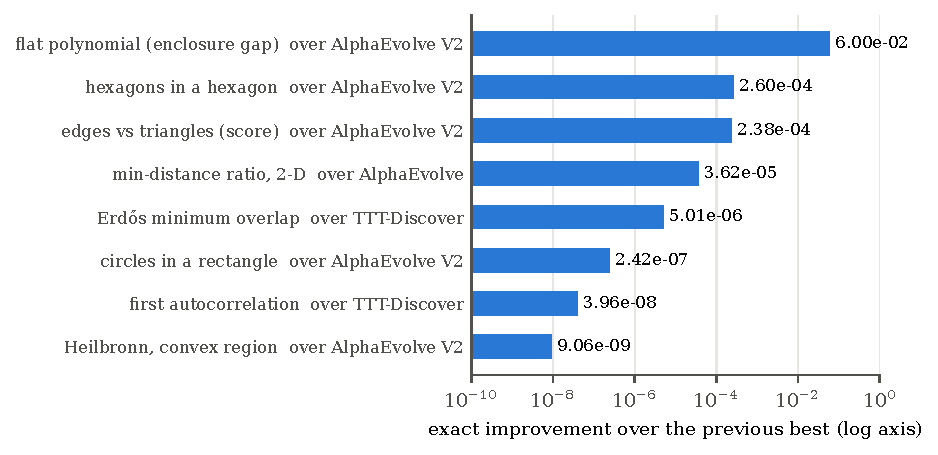
\includegraphics[width=\linewidth]{fig/matmul-records-improvements.pdf}
\caption{The \EAImprovements\ improvements over the previous best, each an exact difference of two
rationals (for the flat polynomial, the gap between two disjoint certified enclosures), on a log axis. All
are positive; the smallest, \EASmallest\ on the Heilbronn configuration, is nine digits in and real. The
largest exact difference, \EALargestExact, is the hexagon side; the benchmark score (edges vs triangles) is
\EdImprovement.}\label{fig:imps}
\end{figure}

\begin{table}[h]\centering\footnotesize
\begin{tabular}{llllp{4.3cm}}\toprule
problem & direction & previous best & exact difference & note \\\midrule
\EAImprovementRows
\bottomrule\end{tabular}
\caption{Every improvement in the table, decided as an exact sign.}\label{tab:imps}
\end{table}

Edges vs triangles is a benchmark score rather than a theorem: rows of twenty weights become (edge density,
triangle density) points by the Newton identities, and the score is the area under the platform's slope-$3$
envelope plus ten times the largest gap in edge density. Recomputed exactly, both printed scores are the
exact values' rounding (\EdPrinted\ rounds \EdExact), and the improvement is \EdImprovement. The Heilbronn
and minimum-distance rows are ratios of exact areas and squared distances; their improvements, \HbImprovement\
and \MdImprovement, are the two smallest in the table and both are real.

\paragraph{Not decided, by name.} Table~\ref{tab:undecided} lists what the ledger refuses. A score estimated
from ten million random samples is not a claim about a construction that exact arithmetic can decide, and
rows of the README with no solution file at the pinned commit are NEEDS DATA: the day the bytes are
published, they are rows. The ledger's battery runs \EABatteryChecks\ checks with \EABatteryReds\ red
controls (an overlapping pair, a box over the perimeter, a collinear triple, a repeated point, a value above
$1$, a zero row, a negative value, a planted touching pair), all firing.

\begin{table}[h]\centering\small
\begin{tabular}{p{2.8cm}p{2.8cm}p{2.2cm}p{6.0cm}}\toprule
problem & the claim & status & why \\\midrule
\EAUndecidedRows
\bottomrule\end{tabular}
\caption{The \EAUndecided\ entries of the table not decided here.}\label{tab:undecided}
\end{table}

\section{What is not claimed}\label{sec:not}

No bound is improved anywhere in this paper and no construction was searched for except the free walk of
Section~\ref{sec:bl}, which beat nothing. Proposition~\ref{prop:at} is not a correction of \cite{Fa22}, which
states the ring; it is the ring dependence decided from the artifact. Proposition~\ref{prop:walls} checks
\LBAttacked\ of \LBNodes\ nodes and says so; the remaining \LBNotAttacked\ rest on the author's reasoning,
which we have no grounds to doubt and have not confirmed. Proposition~\ref{prop:add} verifies the certificate
the authors published, not the search that produced it, not their local optimality searches, and nothing
about the minimum additive cost over all rank-\AddRank\ schemes; \AddCounted\ is an upper bound on a
quantity whose true minimum nobody knows. The $\F_2$ statements of Section~\ref{sec:bl} need not lift to $\Z$
or to any other field, and no lifting was attempted. A REPAIRED row of Section~\ref{sec:ea} is not a
refutation: the platform's tolerance is a design choice and the repaired witness attains the printed value to
nine of ten digits; the flat-polynomial enclosures certify the suprema of two published polynomials, not the
flatness constant; and the benchmark score is defined by the platform's verifier rather than by mathematics.
The sources audited are published, not peer-reviewed; the repository of Section~\ref{sec:ea} carries no
licence file and its bytes are held here for verification only. Nothing here has been sent to any producer.
Finally, the related rank-$48$ $\mm444$ scheme with non-complex coefficients derived from AlphaEvolve's
(arXiv:2506.13242, as recorded in \texttt{notes/alphaevolve-48.md}) is a different artifact and is not in
the corpus.

\cmrepro{The records: \path{certs/strassen-certificate.json} (exported by \CertGeneratedBy),
\path{corpus/strassen-corpus.json} and \path{corpus/alphaevolve-corpus.json} (the converted factors),
\path{corpus/sources/PINS.json} with the pinned \texttt{npz} files, the notebook, the \AddCounted-addition
certificate \path{add55-certificate.json} and Wang's two certificates \path{wang_cert_matrix_q02_n222.pb.txt},
\path{n333.pb.txt}; \path{certs/easota-ledger.json} with \path{corpus/easota/} (\EAFiles\ pinned files, digests in
\path{meta.json}); \path{certs/bilinear-certificate.json} with \path{corpus/bilinear-bounds.json}. The instruments:
\path{instruments/strassen} (\path{tensor.js}; family \path{families/strassen-audit.js}), \path{instruments/tensorlb}
(\path{verify.py}), \path{instruments/slp}, \path{instruments/bilinear} with \path{machine/generate/} (targets, the
flip walk), \path{instruments/easota} (\path{lib.js}, \path{decide.js}, \path{hexagons.js}). The commands:
\texttt{node} \path{tools/paper-numbers/matmul-records.js} writes every macro of this document from those records and refuses if
a record no longer supports a sentence --- in the same run it re-certifies the fast-matmul corpus in-process,
runs \texttt{python3 tools/verify\_strassen.py certs/strassen-certificate.json} (no shared code), re-audits the addition
certificate, re-runs both lower-bound audits, re-decides the \BLTargets\ polynomial schemes, and runs the five batteries
(\texttt{node instruments/strassen/battery.js}, \texttt{node instruments/slp/battery.js},
\texttt{python3 instruments/tensorlb/battery.py}, \texttt{node instruments/easota/battery.js},
\texttt{node instruments/bilinear/battery.js}), all in about ten seconds; \texttt{node tools/run-easota-ledger.js} rebuilds the
EinsteinArena ledger from the pinned bytes; \texttt{node tools/run-bilinear-front.js --targets T8,C8} re-runs a walk;
\texttt{instruments/hseva/.venv/bin/python} \texttt{tools/paper-numbers/matmul-records-figs.py} draws the two
figures from the records; \texttt{node tools/build-paper-tex.js matmul-records} compiles. The report pages \path{reports/alphaevolve.html},
\path{reports/tensor-rank-bounds.html}, \path{reports/matmul-additions.html}, \path{reports/polynomial-multiplication.html}
and \path{reports/easota.html} under \url{https://carlostoledo.co} are built from the same records by builders that
re-run these gates and refuse on any deviation.}

\begin{thebibliography}{99}\small
\bibitem{St69} V.~Strassen, Gaussian elimination is not optimal, \emph{Numer.\ Math.} 13 (1969), 354--356.
\bibitem{Wi71} S.~Winograd, On multiplication of $2\times2$ matrices, \emph{Linear Algebra Appl.} 4 (1971), 381--388.
\bibitem{La76} J.~D.~Laderman, A noncommutative algorithm for multiplying $3\times3$ matrices using 23 multiplications, \emph{Bull.\ Amer.\ Math.\ Soc.} 82 (1976), 126--128.
\bibitem{Br70} R.~P.~Brent, Algorithms for matrix multiplication, Technical Report STAN-CS-70-157, Stanford University, 1970.
\bibitem{Bl03} M.~Bl\"aser, On the complexity of the multiplication of matrices of small formats, \emph{J.\ Complexity} 19 (2003), 43--60.
\bibitem{Wa26} C.~Wang, Automated lower bounds for bilinear complexity over finite fields, arXiv:2603.07280 (2026); certificates at \path{github.com/wcgbg/tensor-rank-lower-bound}, pinned in \path{corpus/sources/}.
\bibitem{Fa22} A.~Fawzi, M.~Balog, A.~Huang, T.~Hubert, B.~Romera-Paredes, M.~Schrittwieser, A.~Novikov, F.~J.~R.~Ruiz, J.~Schrittwieser, G.~Swirszcz, D.~Silver, D.~Hassabis, P.~Kohli, Discovering faster matrix multiplication algorithms with reinforcement learning, \emph{Nature} 610 (2022), 47--53; factorisations \path{alphatensor_r.npz}, \path{alphatensor_f2.npz} of \path{github.com/google-deepmind/alphatensor}, pinned.
\bibitem{No25} A.~Novikov et al., AlphaEvolve: a coding agent for scientific and algorithmic discovery, arXiv:2506.13131 (2025); the decomposition is in \path{mathematical_results.ipynb} of \path{github.com/google-deepmind/alphaevolve_results}, pinned at commit \AECommit.
\bibitem{GGTW25} B.~Georgiev, J.~G\'omez-Serrano, T.~Tao, A.~Z.~Wagner, arXiv:2511.02864 (2025) --- the ``AlphaEvolve V2'' constructions, as recorded in the ledger.
\bibitem{KM22} M.~Kauers, J.~Moosbauer, Flip graphs for matrix multiplication, arXiv:2212.01175 (2022).
\bibitem{CK25} S.~Chen, M.~Kauers, Flip graphs for polynomial multiplication, arXiv:2502.06264 (2025).
\bibitem{KI26} Karunaratne and Idamekorala, arXiv:2607.28676 (July 2026), with the certificate \path{add55-certificate.json} as pinned in \path{corpus/sources/}; cited as recorded in \path{reports/matmul-additions.html}.
\bibitem{EA26} Together AI, \emph{EinsteinArena-new-SOTA}, \path{github.com/togethercomputer/EinsteinArena-new-SOTA}, commit \EACommit, fetched \EAFetched; the constructions and READMEs as pinned in \path{corpus/easota/}.
\bibitem{TTT26} Yuksekgonul et al., TTT-Discover, arXiv:2601.16175 (2026), as recorded in the ledger.
\bibitem{Ha16} J.~K.~Haugland, The minimum overlap problem revisited, arXiv:1609.08000 (2016).
\bibitem{Wi77} S.~Winograd, Some bilinear forms whose multiplicative complexity depends on the field of constants, \emph{Math.\ Systems Theory} 10 (1977), 169--180.
\bibitem{WM83} M.~D.~Wagh, S.~D.~Morgera, A new structured design method for convolutions over finite fields, part I, \emph{IEEE Trans.\ Inform.\ Theory} 29 (1983), 583--595.
\bibitem{Mo90} S.~D.~Morgera, Multiplicative complexity of bilinear algorithms for cyclic convolution over finite fields, \emph{Multidimensional Systems and Signal Processing} 1 (1990), 99--111.
\bibitem{Mo05} P.~L.~Montgomery, Five, six, and seven-term Karatsuba-like formulae, \emph{IEEE Trans.\ Computers} 54 (2005), 362--369.
\bibitem{FH07} H.~Fan, M.~A.~Hasan, Comments on ``Five, six, and seven-term Karatsuba-like formulae'', \emph{IEEE Trans.\ Computers} 56 (2007), 716--717.
\bibitem{CO11} M.~Cenk, F.~\"Ozbudak, Multiplication of polynomials modulo $x^n$, \emph{Theoret.\ Comput.\ Sci.} 412 (2011), 3451--3462.
\bibitem{Kiss} C.~Toledo, Two platforms, one configuration: independent exact certification of the dimension-eleven kissing records, draft (September 2026), \path{paper/tex/kissing-ledger.tex} of this repository.
\end{thebibliography}

\end{document}
